% Header
\noindent
{\small\textsf{\textbf{MỤC 4.4}}\hspace{1.5em}\textsf{Các dạng vô định và quy tắc l’Hospital}}\hfill{\small\textbf{315}}
\vspace{1em}
\hrule height 0pt
\vspace{0.5em}

\noindent
\begin{minipage}[t]{46mm}
\vspace{0pt}
\footnotesize
\vspace{5.8cm}

Mặc dù các dạng kiểu $0^0$, $\infty^0$ và $1^\infty$ là vô định, nhưng dạng $0^\infty$ không phải là dạng vô định. (Xem Bài tập 88.)

\vspace{5.0cm}

Đồ thị của hàm số $y = x^x$, $x > 0$, được thể hiện trong Hình~6. Lưu ý rằng mặc dù $0^0$ không được xác định, các giá trị của hàm số tiến dần về 1 khi $x \to 0^+$. Điều này khẳng định kết quả của Ví dụ~10.

\vspace{0.8em}
\centering
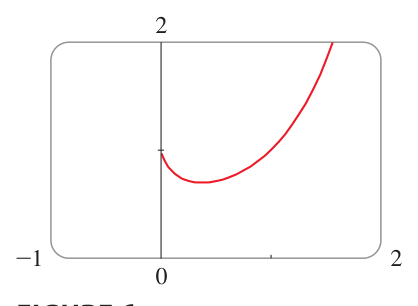
\includegraphics[width=\linewidth]{images/p0350_fig1.png}
\vspace{0.3em}

{\bfseries\color{stewartblue}HÌNH 6}
\end{minipage}\hfill
\begin{minipage}[t]{126mm}
\vspace{0pt}
Số hạng $e^x/x \to \infty$ khi $x \to \infty$ theo quy tắc l’Hospital và vì thế bây giờ ta có một tích mà trong đó cả hai thừa số đều tăng vô hạn:
\[
\lim_{x \to \infty} (e^x - x) = \lim_{x \to \infty} \left[ x \left( \frac{e^x}{x} - 1 \right) \right] = \infty \qquad \textcolor{stewartblue}{\blacksquare}
\]

\vspace{0.8em}
\noindent{\color{stewartblue}\rule{1.1ex}{1.1ex}}\hspace{0.5em}\textbf{\large Các dạng lũy thừa vô định (Dạng $0^0$, $\infty^0$, $1^\infty$)}

Một số dạng vô định phát sinh từ giới hạn
\[
\lim_{x \to a} [f(x)]^{g(x)}
\]
\vspace{-0.5em}
\begin{center}
\renewcommand{\arraystretch}{1.3}
\begin{tabular}{@{}llll@{}}
\textbf{1.} & $\lim\limits_{x \to a} f(x) = 0$ & \quad và \quad $\lim\limits_{x \to a} g(x) = 0$ & \qquad dạng $0^0$ \\
\textbf{2.} & $\lim\limits_{x \to a} f(x) = \infty$ & \quad và \quad $\lim\limits_{x \to a} g(x) = 0$ & \qquad dạng $\infty^0$ \\
\textbf{3.} & $\lim\limits_{x \to a} f(x) = 1$ & \quad và \quad $\lim\limits_{x \to a} g(x) = \pm\infty$ & \qquad dạng $1^\infty$
\end{tabular}
\end{center}

Mỗi trường hợp trong ba trường hợp này đều có thể được xử lý bằng cách lấy logarit tự nhiên:
\[
\text{đặt}\quad y = [f(x)]^{g(x)}, \quad \text{khi đó}\quad \ln y = g(x) \ln f(x)
\]
hoặc bằng cách sử dụng Công thức 1.5.10 để viết hàm số dưới dạng hàm mũ:
\[
[f(x)]^{g(x)} = e^{g(x) \ln f(x)}
\]
(Hãy nhớ lại rằng cả hai phương pháp này đều đã được sử dụng khi tính đạo hàm của các hàm số dạng này.) Trong cả hai phương pháp, ta đều được dẫn tới tích vô định $g(x) \ln f(x)$, thuộc dạng $0 \cdot \infty$.

\vspace{0.6em}
\noindent\textbf{\color{stewartblue}VÍ DỤ 9}\hspace{1em}Tính $\lim\limits_{x \to 0^+} (1 + \sin 4x)^{\cot x}$.

\noindent\textbf{\color{stewartblue}LỜI GIẢI}\hspace{1em}Trước hết hãy lưu ý rằng khi $x \to 0^+$, ta có $1 + \sin 4x \to 1$ và $\cot x \to \infty$, do đó giới hạn đã cho là vô định (dạng $1^\infty$). Đặt
\[
y = (1 + \sin 4x)^{\cot x}
\]
Khi đó
\[
\ln y = \ln [(1 + \sin 4x)^{\cot x}] = \cot x \ln (1 + \sin 4x) = \frac{\ln(1 + \sin 4x)}{\tan x}
\]
vì vậy quy tắc l’Hospital cho ta
\[
\lim_{x \to 0^+} \ln y = \lim_{x \to 0^+} \frac{\ln(1 + \sin 4x)}{\tan x} = \lim_{x \to 0^+} \frac{\dfrac{4\cos 4x}{1 + \sin 4x}}{\sec^2 x} = 4
\]
Cho đến đây chúng ta mới chỉ tính giới hạn của $\ln y$, nhưng điều chúng ta muốn là giới hạn của $y$. Để tìm điều này, chúng ta sử dụng sự kiện $y = e^{\ln y}$:
\[
\lim_{x \to 0^+} (1 + \sin 4x)^{\cot x} = \lim_{x \to 0^+} y = \lim_{x \to 0^+} e^{\ln y} = e^4 \qquad \textcolor{stewartblue}{\blacksquare}
\]

\vspace{0.6em}
\noindent\textbf{\color{stewartblue}VÍ DỤ 10}\hspace{1em}Tìm $\lim\limits_{x \to 0^+} x^x$.

\noindent\textbf{\color{stewartblue}LỜI GIẢI}\hspace{1em}Lưu ý rằng giới hạn này là vô định vì $0^x = 0$ với mọi $x > 0$ nhưng $x^0 = 1$ với mọi $x \neq 0$. (Hãy nhớ rằng $0^0$ không xác định.) Chúng ta có thể tiến hành như trong Ví dụ 9 hoặc bằng cách viết hàm số dưới dạng hàm mũ:
\[
x^x = (e^{\ln x})^x = e^{x \ln x}
\]
\end{minipage}
